\documentclass[a4paper]{article}
\usepackage[margin=1.5in, width=6in]{geometry}
\usepackage{graphicx, subcaption}
\usepackage{amssymb, amsmath, amsthm}
\usepackage{amsthm}
\usepackage{xcolor}
\usepackage{babel}
\usepackage{hyperref}
\usepackage{parskip}

\renewcommand{\d}{\mathrm{d}}
\newcommand{\pfrac}[2]{\left(\frac{#1}{#2}\right)}
\newcommand{\bfrac}[2]{\left[\frac{#1}{#2}\right]}
\begin{document}
	
\section*{Objective}
\textbf{Characterization of the DPD metric with respect to tuning parameter $\alpha$.} Given an $\alpha$ in a minimal Density Power Divergence fitting setup, can I analytically say if the optimal fit will be robust or efficient?

\textbf{Details:}
\begin{enumerate}
	\item I want to fit a candidate distribution $f(x; \theta)$ over a target density $g(x; \theta)$ possibly contaminated with outliers, by minimizing the $DPD_\alpha(f, g)$ divergence over $\theta \in \Theta$.
	\item Suppose we partition parameter space $\Theta$ of the candidate density into
	\[\Theta = \Theta_r \cup \Theta_e\]
	viz. robust and efficient estimates.
	\item I intend to find the partitions of $A = [0,1] \ni \alpha$:
	\[A = A_r \cup A_e\]
	which cause the robust and efficient fits respectively. i.e. upon selecting $\alpha \in A_r$, we obtain min. div. estimate $\theta \in \Theta_r$.
\end{enumerate}

\textbf{I'm hoping this will answer a long-standing question of selection of the tuning parameter for DPD.}

\section*{Progress}
I have devised a visualization that I call the ``potential map''. See \autoref{fig:dpdpots}

DPD divergence is some integral
\[D(f,g): \int_{x \in \mathcal X} L(f(x),g(x)) \d x \]

Call $V(x,y) = L(y, g(x))$ the \textbf{divergence potential associated with $g$ and induced by $L$} (probably bad nomenclature! Some source called it ``divergence density'', not sure if that is standard terminology).

Plotting $V$ (either 3D map or heat-plot) gives a glimpse at the ``topography of penalization of $D(\cdot, \cdot)$ with respect to $g$'', because I think
\begin{quote}
	The process of fitting a candidate distribution over a given target is merely an act of minimizing the line integral of the potential function $V(x,y)$ along the density line $f(x; \theta)$, where the minimization is over $\Theta$.
\end{quote}

I say line integral but it is not exactly line integral per se.

I have tabulated common divergences with their associated potentials are provided in \autoref{tab:pdfpotlist}. Note how these divergences are functions of $f-g$, i.e. dependent on the abscissa-wise deviation of the candidate density from the target. However the \textbf{rate of increment of penalization} with increasing abscissa-wise deviation are functionally different across different divergence metrics. Further, for DPD, it is also controllable by its hyperparameter $\alpha$.

\begin{table}[h!]
	\begin{tabular}{c|c|c|c}
		Divergence name  &  Form  &  Potential $L_g(y)$  &  Gradient $\nabla_y L_g(y)$\\
		\hline \vspace{0.1cm}
		Hellinger  &  $\int \frac{1}{2} (\sqrt{f(x)} - \sqrt{g(x)})^2 \d x$  &  $\frac{1}{2} (\sqrt y - \sqrt g)^2$  &  $\frac{1}{2 \sqrt y} (\sqrt y - \sqrt g)$\\
		DPD-\texorpdfstring{$\alpha$}{alpha}  &  $\int f^\alpha(f-g) - \frac{1}{\alpha}g(f^\alpha - g^\alpha) \d x$  &  $f^\alpha(f-g) - \frac{1}{\alpha}g(f^\alpha - g^\alpha)$  &  $(1+\alpha) y^{\alpha-1} (y-g)$\\
	\end{tabular}
	\caption{Some common PDF-PDF divergences and their potential functions}
	\label{tab:pdfpotlist}
\end{table}


\subsection*{A graphical demonstration}

\begin{figure}[h]
	\begin{subfigure}{0.49\linewidth}
		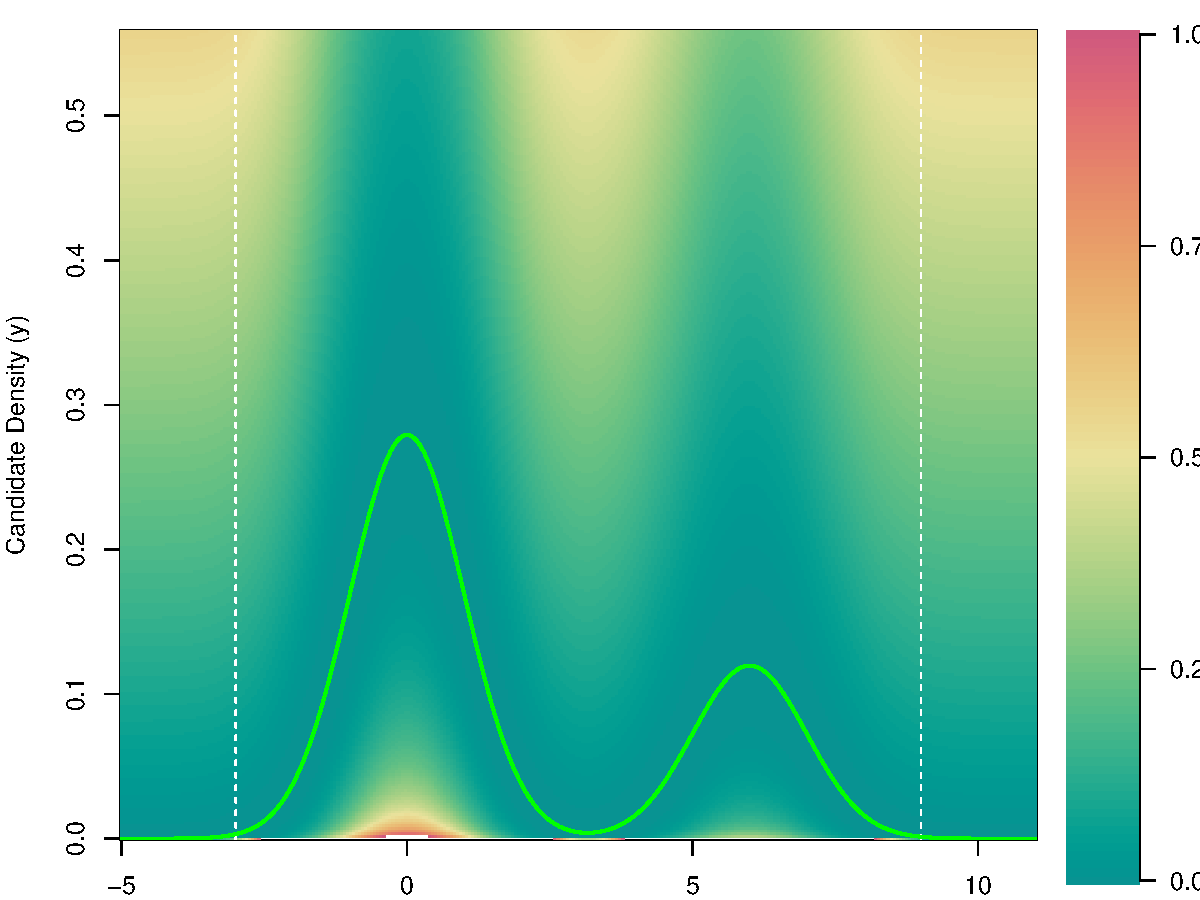
\includegraphics[width=\linewidth]{fig/divpot contamin 0.01}
		\caption{$\alpha=0.01$}
	\end{subfigure}
	\begin{subfigure}{0.49\linewidth}
		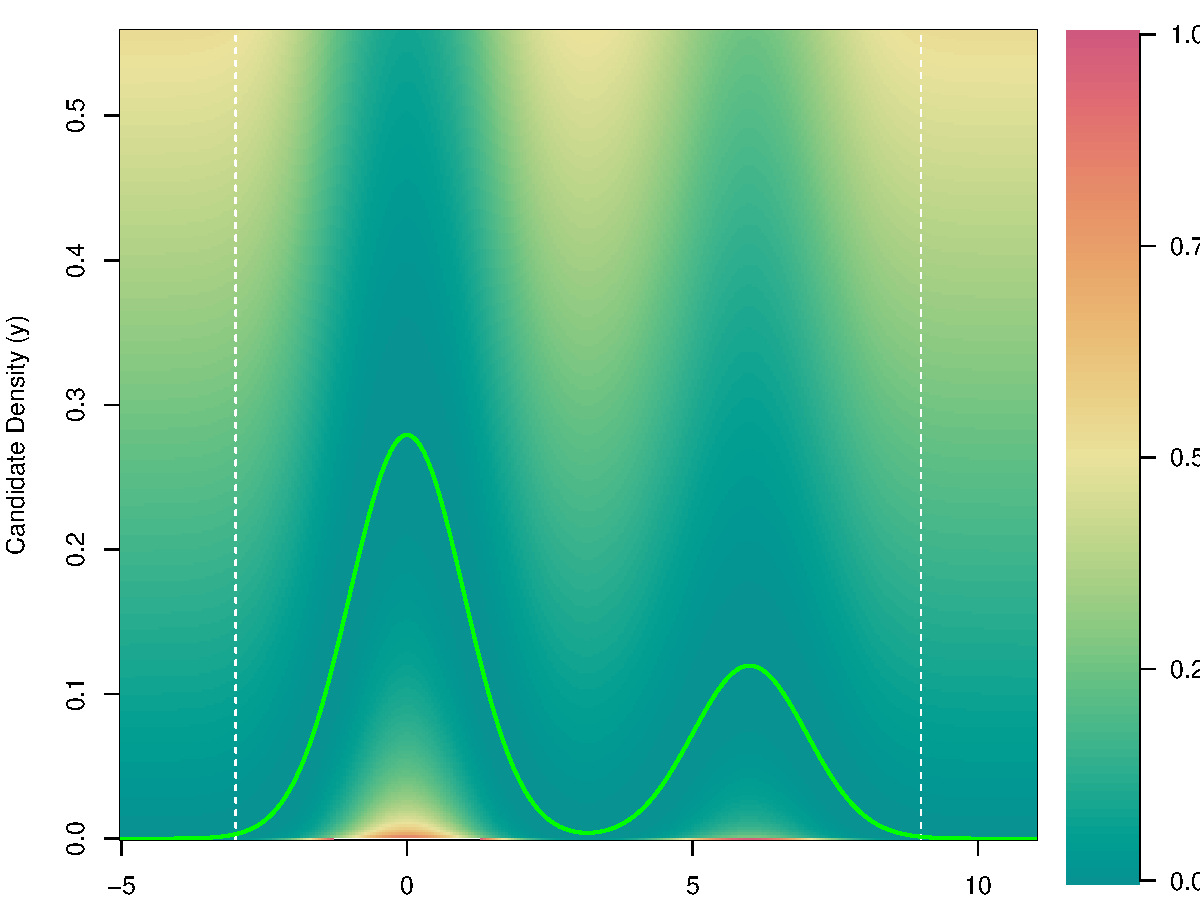
\includegraphics[width=\linewidth]{fig/divpot contamin 0.1}
		\caption{$\alpha=0.1$}
	\end{subfigure}
	\begin{subfigure}{0.49\linewidth}
		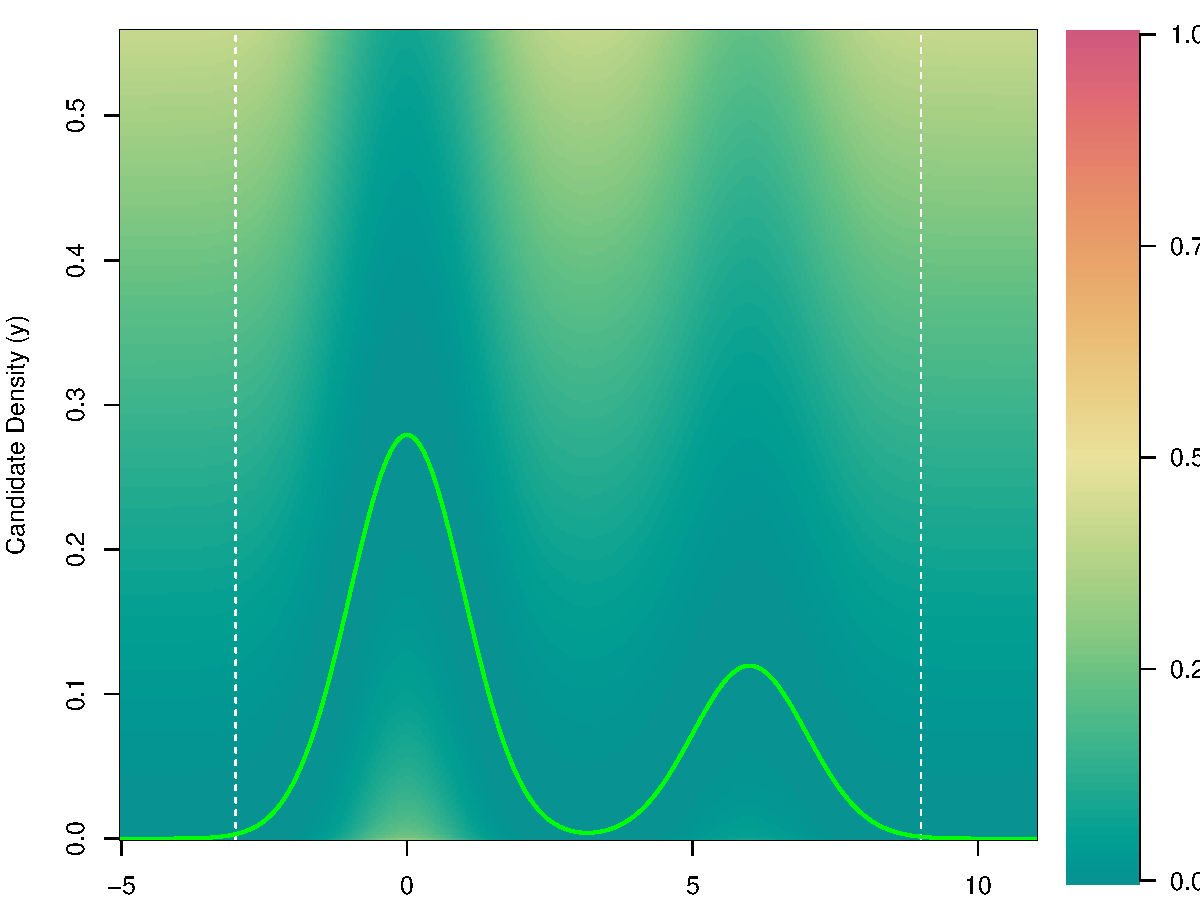
\includegraphics[width=\linewidth]{fig/divpot contamin 0.5}
		\caption{$\alpha = 0.5$}
	\end{subfigure}
	\begin{subfigure}{0.49\linewidth}
		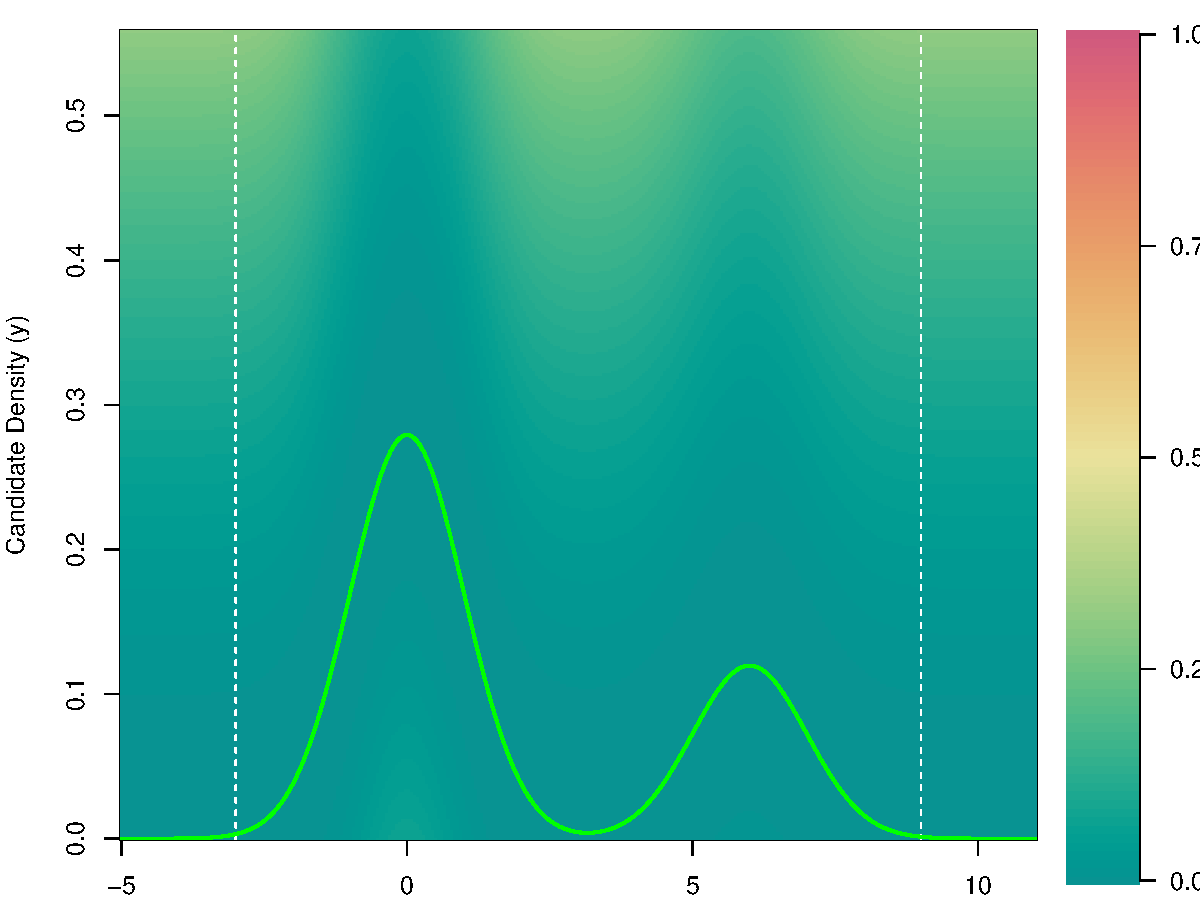
\includegraphics[width=\linewidth]{fig/divpot contamin 1}
		\caption{$\alpha = 1$}
	\end{subfigure}
	\caption{Divergence Potentials created by the same contaminated density for different $\alpha$'s of DPD}
	\label{fig:dpdpots}
\end{figure}

\textbf{Observation:}\\
If we were to fit (via say numerical optimization) some unimodal $f$ over this contaminated $g$, we would expect to see that:

\begin{enumerate}
	\item Higher $\alpha$ induces lower penalization for deviating some amount from the target $g$, thereby making an efficient fit that spans over both density peaks more feasible.
	
	\item However, a lower $\alpha$ allows isolated fitting over one of the 2 peaks only (the principal peak fares better), since otherwise, trying to span both peaks by passing through the middle high-penalization region incurs a lot of penalty/potential.
\end{enumerate}

\textbf{Important Takeaway}\\
For contaminated densities, it is not the ``attraction'' of the second peak that deviates the candidate to fit contaminatedly (i.e. efficiently), but it is the high potential ``hill'' in between that discourages such a fit.

\textbf{Example Formulation:}\\
Let $f(x; a,d,s,k) := \frac{1}{dA(s,k)} \sin^k \pfrac{x-a}{d}^s$ with $a,d,s,k$ all unknown,\\
$g(x) := p \phi(x) + (1-p) \phi(x-h)$ with $p, h$ given,\\
and for a given $\alpha$, the task is to minimize:
\[\min_{s,k} \int_a^{a+d} \left[f^\alpha(x) (f-g)(x) - \frac{1}{\alpha} g(x) (f^\alpha - g^\alpha)(x) \right] \d x \]

\end{document}